
%{{{ Preamble

%\documentclass[draft]{beamer} %% normal document
\documentclass[]{beamer} %% normal document
\usepackage{fontspec, unicode-math, caption, float, filecontents, verbatim}
\usepackage[english]{babel}

%{{{ Beamer Stuff

\usetheme{Frankfurt}
\useoutertheme{split}
\useinnertheme{rectangles}
%%\definecolor{bettergreen}{rgb}{.1,.7,.1}
%%\usecolortheme[named=bettergreen]{beaver}

\definecolor{bettergreen}{rgb}{0.1,0.7,0.1}

%\usetheme{Dresden}
%\usecolortheme[named=bettergreen]{structure}
\usecolortheme[named=bettergreen]{structure}

\setbeamercolor{section in head/foot}{fg=green, bg=black}
\setbeamercolor{section shaded}{fg= grey}


%\setbeamertemplate{caption}[numbered]
%\captionsetup{labelformat=simple,font=scriptsize,labelfont=scriptsize}
\beamertemplatenavigationsymbolsempty

% puts Frame numbers in Dresden template
\newcommand*\oldmacro{}%
\let\oldmacro\insertshorttitle%
\renewcommand*\insertshorttitle{%
	\oldmacro\hfill%
\insertframenumber\,/\,\inserttotalframenumber}

%\logo{\pgfimage[width=2cm,height=2cm]{material/schlangenlogo}}
\newcommand{\nologo}{\setbeamertemplate{logo}{}} % command to set the logo to nothing


\AtBeginSection[]
{%
	\begin{frame}<beamer>
		\frametitle{Table of Contents}
		\tableofcontents[currentsection]
		%\tableofcontents
	\end{frame}
}




%}}}

\newcommand{\as}[1]{{\fontspec{ProFontWindows} \textcolor{white}{#1} } }
\newcommand{\source}[1]{{\caption{\tiny {\fontspec{ProFontWindows} {Source: #1} } } } }
\newcommand{\greenbullet}{\textcolor{bettergreen}\textbullet}
%\newcommand{\greencirc}{\textcolor{bettergreen} $ \circ $}
\newcommand{\greencirc}{$ \circ $ }

\usepackage{multicol}

\usepackage{tikz}
\usetikzlibrary{arrows, decorations.markings}
\usetikzlibrary{positioning,shapes,shadows,calc,positioning}
\usetikzlibrary{decorations.pathreplacing,angles,quotes}
\usetikzlibrary{decorations.pathmorphing}
%\usetikzlibrary{fit}


% This part taken from http://www.texample.net/tikz/examples/double-arrows/
% Double Arrows a la Chef
% Author: Dominik Haumann

% for double arrows a la chef
% adapt line thickness and line width, if needed
%\tikzstyle{vecArrow} = [thick, decoration={markings,mark=at position
%   1 with {\arrow[semithick]{open triangle 60}}},
%   double distance=1.4pt, shorten >= 5.5pt,
%   preaction = {decorate},
%   postaction = {draw,line width=1.4pt, white,shorten >= 4.5pt}]
%\tikzstyle{innerWhite} = [semithick, white,line width=1.4pt, shorten >= 4.5pt]


%\tikzstyle{mynode} = [rectangle,rounded corners,draw=black,top color=white, bottom color=white!50,very thick, inner sep=1em, minimum size=3em, text centered]
%\tikzstyle{invnode} = [inner sep=0,minimum size=0]
%
%\tikzstyle{abstract}=[rectangle, draw=black, rounded corners, fill=blue!40, drop shadow, text centered, anchor=north, text=white, text width=3cm]
%\tikzstyle{comment}=[rectangle, draw=black, rounded corners, fill=green, drop shadow, text centered, anchor=north, text=white, text width=3cm]
%\tikzstyle{myarrow}=[->, >=open triangle 90, thick]
%\tikzstyle{line}=[-, thick]


\tikzset{font={\fontsize{8pt}{7}\selectfont}}
\tikzset{every picture/.append style={scale=0.1}}


\usepackage{etex} %% Cool Stuff, see http://tex.stackexchange.com/a/36721/69074 : \foreach \i in {0,...,\number\numexpr\memBlocks-1\relax}
\newcommand{\CC}{C\nolinebreak\hspace{-.05em}\raisebox{.4ex}{\tiny\bf +}\nolinebreak\hspace{-.03em}\raisebox{.4ex}{\tiny\bf +}}




%{{{ Extract Coordinates

% http://tex.stackexchange.com/a/179946/69074
\makeatletter
\def\extractcoord#1#2#3{%
  \path let \p1=(#3) in \pgfextra{%
    \pgfmathsetmacro#1{\x{1}/\pgf@xx}%
    \pgfmathsetmacro#2{\y{1}/\pgf@yy}%
    \xdef#1{#1} \xdef#2{#2}%
  };%
}%
\makeatother

\newcommand*{\LabelCoord}[4]{\fill [#1] ($(#2,#3)$) circle (2pt) node [right] {#4}}%
%}}}


% For image1
\newif\iffourway

% For image3
\newif\ifshowreq
\newif\ifshowwb





%{{{ inputfile

% source: http://tex.stackexchange.com/questions/40738/how-to-properly-make-a-latex-project
\newcommand\inputfile[1]{%
    \InputIfFileExists{#1}{}{\typeout{No file #1.}}%
}


%\newcommand*{\COMPILEIMAGES}{}%


% Whether to compile the image-lets or include the pre-compiled ones
\newcommand*{\COMPILEIMAGES}{}%

\newcommand\inputimage[1]}}

%{{{ Avebritations

\usepackage{xspace}
\newcommand{\twi}{I\textsuperscript{2}C\xspace}
\newcommand{\mosi}{\texttt{MOSI}\xspace}
\newcommand{\miso}{\texttt{MISO}\xspace}
\newcommand{\clock}{\texttt{CLOCK}\xspace}
\renewcommand{\ss}{\texttt{\textoverline{SS}}\xspace}

\newcommand{\sda}{\texttt{SDA}\xspace}
\newcommand{\scl}{\texttt{SCL}\xspace}
\newcommand{\startcondition}{\texttt{START} condition\xspace}
\newcommand{\stopcondition}{\texttt{STOP} condition\xspace}
\newcommand{\clockstretching}{\texttt{CLOCK STRETCHING}\xspace}
\newcommand{\ack}{\texttt{ACK}\xspace}
\newcommand{\nak}{\texttt{NACK}\xspace}
%}}}

%{{{ MINTED

\usepackage{minted}
\definecolor{bg}{rgb}{0.95,0.95,0.95}
%\newminted[C++]{cpp}{numbersep=5pt, bgcolor=bg, gobble=0, linenos, tabsize=4}
%\newminted[C++]{cpp}{tabsize=4, obeytabs}
%}}} Minted

%{{{ Hyperref

\usepackage{hyperref}
\definecolor{darkblue}{rgb}{0,0,.5}
%linkcolor will also affect the text in the navigation bar on the top of each slide
%\hypersetup{pdftex=true, colorlinks=true, breaklinks=true, linkcolor=darkblue, menucolor=darkblue, pagecolor=darkblue, urlcolor=darkblue}
\hypersetup{pdfpagemode=FullScreen}
%}}}

%{{{ Animate

%%\usepackage[controls, autoplay]{animate}
%\usepackage[autoplay]{animate}
%%\animategraphics[<options>]{<frameand the environment rate>}{<file basename>}{<first>}{<last>}
%}}}

%{{{ Changemargin

\newenvironment{changemargin}[2]
{
	\begin{list}{}
		{
			\setlength{\topsep}{0pt}
			\setlength{\leftmargin}{#1}
			\setlength{\rightmargin}{#2}
			\setlength{\listparindent}{\parindent}
		\setlength{\itemindent}{\parindent}
			\setlength{\parsep}{\parskip}
		}
	\item[]
	}
	{
	\end{list}
}
%}}}

%{{{ Graphics Loading

\usepackage{graphicx}
\graphicspath{{../material/presentation/}{../material/background/}}
\usepackage{caption}
\captionsetup[figure]{labelformat=empty, font=scriptsize, justification=raggedleft, singlelinecheck=false}% redefines the caption setup of the figures environment in the beamer class.
%}}}

%{{{ Tkz drawing package

%{{{ Spider diagram

%\usepackage{tkz-kiviat,numprint,fullpage}
\usepackage{tkz-kiviat,numprint}
\usetikzlibrary{arrows}
%}}}

%{{{ Block diagram

\usepackage{tikz}
\usetikzlibrary{arrows, decorations.markings, positioning}

% for double arrows a la chef
% adapt line thickness and line width, if needed
\tikzstyle{vecArrow} = [thick, decoration={markings,mark=at position
	1 with {\arrow[semithick]{open triangle 60} } },
	double distance=1.4pt, shorten >= 5.5pt,
	preaction = {decorate},
postaction = {draw,line width=1.4pt, white,shorten >= 4.5pt}]
\tikzstyle{innerWhite} = [semithick, white,line width=1.4pt, shorten >= 4.5pt]
%}}}

%{{{ Tkz timing package

\usepackage{tikz-timing}
%\usetikztiminglibrary{nicetabs} % a bit strange with \Huge; use belowrulesep to adjust
%}}}

%}}}

%{{{ Fullpage

\newenvironment{fullpage}[0]{%
	\begin{list}{}{%
		\setlength{\leftmargin}{-10mm}%
		\setlength{\rightmargin}{-10mm}%
		\vspace*{-10pt}
		}%
\item[]}{\end{list}}
%}}}


%{{{ Title

\title[]{RISC V - Architecture and Interfaces}
\subtitle[]{The RocketChip}
%\subject{}
\keywords{RISCV, RocketChip}
\date{\today}
%}}}

%{{{ Author

\author{Moritz~Nöltner-Augustin}
\institute[ZITI]}}

%}}}




%{{{
\begin{document}

%{{{ Titlepage

\begin{frame}[plain]
	\titlepage
	%\note{}
\end{frame}
%}}}

%{{{ Table of Contents

\begin{frame}<beamer>
	\frametitle{Table of Contents}
	\tableofcontents
\end{frame}
%}}}




%{{{
\section{Introduction}

%{{{
\begin{frame}{What is RISCV?}
	Open source ISA...
\end{frame}
%}}}

%{{{
\begin{frame}{What is RocketChip?}
	\centering
	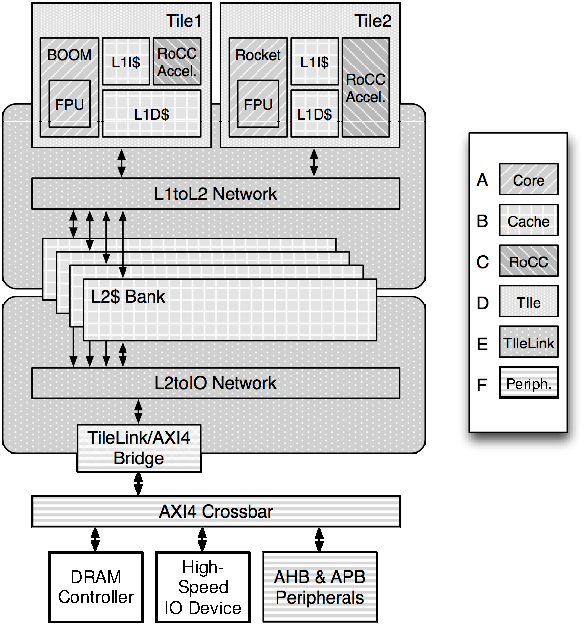
\includegraphics[width=0.90\pagewidth,height=0.80\pageheight,keepaspectratio]{EECS-2016-17_fig1}
\end{frame}
%}}}

%{{{
\begin{frame}[fragile]{How can I "use" RocketChip?}
	\begin{minipage}[c][.4\textheight][c]{\linewidth}
		\begin{minted}[fontsize=\small, gobble=3]{bash}
			git clone https://github.com/ucb-bar/rocket-chip.git
			cd rocket-chip
			#git checkout boom
			git submodule update --init --recursive
			# Now the repo is about 3GB
			cd riscv-tools
			export RISCV=/path/to/toolchain/install
			export PATH="${PATH}:$RISCV/bin"
			./build.sh # Takes about 45 min
			# The toolchain is another 800MB
			cd ../emulator
			make run CONFIG=BOOMConfig
			make run CONFIG=ExampleSmallConfig
			cd ../vsim
			make -jN CONFIG=ExampleSmallConfig # about 20 min
		\end{minted}
	\end{minipage}
\end{frame}
%}}}

%}}} End: section{Introduction}


%{{{
\section{Structure}

%{{{
\begin{frame}[fragile]{What can be configured?}
	\$(ROCKET-CHIP)/src/main/scala/coreplex/Configs.scala:
	\begin{columns}
		\column{0.33\textwidth}
		More than 70 parameters:
		\begin{itemize}
			\item MemWidth
			\item Cache (I \& D)
				\begin{itemize}
					\item nSets
					\item nWays
					\item rowBits
					\item nTLBEntries
					\item cacheIdBits
					\item splitMetadata
					\item Replacer
				\end{itemize}
			\item NBreakpoints
			\item FPUKey
			\item UseAtomics
		\end{itemize}
		\pause
		\column{0.67\textwidth}
		\begin{minted}[fontsize=\small, gobble=3, tabsize=2]{java}
			pname match {
				case PAddrBits => 32
				case NTiles => 1
				...
			}
		\end{minted}
		\pause
		\begin{minted}[fontsize=\small, gobble=3, tabsize=2]{java}
			...
			class WithNCores(n: Int) extends Config(
				(pname,site,here) => pname match {
					case NTiles => n
					case _ => throw new CDEMatchError
				})
		\end{minted}
		\pause
		\begin{minted}[fontsize=\small, gobble=3, tabsize=2]{java}
			...
			class DualCoreConfig extends Config(
			new WithNCores(2) ++ new WithL2Cache
			                  ++ new BaseConfig)
		\end{minted}
	\end{columns}
\end{frame}
%}}}


%{{{
\begin{frame}[fragile]{How can I configure the chip?}
	\begin{minted}[fontsize=\small, gobble=1, tabsize=2]{java}
	class BaseCoreplexConfig extends Config ((site, here, up) => {
		case CacheName("L1I") => CacheConfig(
			nSets         = 64,
			nWays         = 4,
			rowBits       = site(L1toL2Config).beatBytes*8,
			nTLBEntries   = 8,
			cacheIdBits   = 0,
			splitMetadata = false)
	\end{minted}
	\pause
	\begin{minted}[fontsize=\small, gobble=1, tabsize=2]{java}
	...
	class WithL1ICacheSets(sets: Int)
		extends Config((site,here,up) => {
		case CacheName("L1I") =>
			up(CacheName("L1I"),site).copy(nSets=sets)
	})
	\end{minted}
	\pause
	\begin{minted}[fontsize=\small, gobble=1, tabsize=2]{java}
	...
	class DualCoreConfig2way32sets extends Config(
		new WithNCores(2)++new WithL1ICacheSets(32)++new BaseConfig)
	\end{minted}
\end{frame}
%}}}


%{{{
\begin{frame}{How to add configuration?}
	\begin{fullpage}
		\centering
		\inputimage{image1}
	\end{fullpage}
\end{frame}
%}}}

%}}} End: section{Structure and Interfaces}


%{{{
\section{Interfaces}

%{{{
\begin{frame}{AXI-Interface}
	Note: AXI4... does not mean axi for ... but is the protocol version, AXI4.
	TODO
\end{frame}
%}}}

%{{{
\begin{frame}{Title}
	TODO
\end{frame}
%}}}

%}}} End: section{Structure and Interfaces}


%{{{
\section[Conclusion]{Conclusion}


%{{{
\begin{frame}[fragile]{Comparison of SPI an \twi}
\end{frame}
%}}}

%}}} End: section{}





%{{{ References

\center{References}
\tiny
\begin{thebibliography}{9}
	\bibitem{spi_mc68hc11a8}
		Datasheet of the Motorola MC68HC11A8 microcontroller describing the SPI bus.\\
		Last downloaded 2014-01-10\\
		\url{http://cache.freescale.com/files/microcontrollers/doc/data_sheet/MC68HC11A8.pdf}

\end{thebibliography}
%}}}

%{{{ END

\begin{frame}
	{\Huge End}
	Any Questions?
\end{frame}
%}}}

\end{document}
%}}}
